\documentclass[twocolumn]{article}
\usepackage{graphicx}
% \usepackage{hyperref}
\usepackage{tcolorbox}
\usepackage{parskip}
\usepackage{enumitem}
\usepackage[numbers]{natbib}
\usepackage{mdframed}
\usepackage[margin=0.8in]{geometry}
\usepackage{amsmath}
\usepackage{amsfonts}
\usepackage{subcaption}
\usepackage{dblfloatfix}
\usepackage{placeins}
\usepackage{url}
\def\UrlBreaks{\do\/\do-}
\usepackage[colorlinks=true, linkcolor=blue, citecolor=blue, urlcolor=blue]{hyperref}

\title{\textbf{Bayesian Image Super-Resolution: \\Replicated Results}}
\author{Marcus Bluestone \\ \texttt{marcusbl@mit.edu}}
\date{May 5, 2026}

\begin{document}
\setlist[enumerate,1]{label*=\arabic*.}

\maketitle

\section{Introduction}
Image Super-Resolution (SR) is the task of recovering a high-resolution (HR) image from multiple noisy, downsampled, and misaligned low-resolution (LR) observations. This project replicates the framework presented in \textit{Bayesian Image Super-Resolution} \cite{tipping2003}, which proposes a novel Bayesian methodology for SR. 

In traditional Maximum A Posteriori (MAP) approaches, the HR image and the registration parameters are estimated simultaneously \cite{hardie1997}. However, this may lead to poor reconstruction and possibly biased or overfit results. The Bayesian approach improves upon this by marginalizing out the HR image, allowing the registration parameters to be optimized independently. 

The primary objectives of this replication are:
\begin{itemize}
    \item \textbf{Implementation:} Translating the original probabilistic framework into a modern computational pipeline leveraging PyTorch and GPU acceleration. 
    \item \textbf{Structural Clarity:} Providing detailed geometric visualizations (Figures \ref{fig:grid} and \ref{fig:shift_grid}) and mathematical derivations to clarify the spatial transformation and pixel-mapping logic only briefly described in the original text. 
    \item \textbf{Replicability and Open Science:} Contributing a modular, open-source implementation to facilitate further research. The complete code and experiments are available at \url{https://github.com/MarcusBluestone/BayesianSuperResolution}. 
\end{itemize}
\section{Methodology}
In this section, we detail the precise procedure used to create the LR images and reconstruct the HR image using the MAP and Bayes methods. 

\subsection{Setup}
To align with the paper's notation, we rasterize (by column) all images into column vectors. 

We define the HR image as $x \in \mathbb{R}^N$ and each of the $K$ LR images as $y^{(k)}\in \mathbb{R}^M$ for $k \in \{1, \dots, K\}$. The goal is to produce an estimate $\hat{x} \in \mathbb{R}^N$ that is close to the original $x$. 

We index the pixels in the HR image by $i \in \{1, \dots, N\}$ and the pixels in the LR images by $j \in \{1, \dots, M\}$. We define $v_i \in \mathbb{R}^2$ as the spatial coordinate of the $i$-th pixel in the HR image. Similarly, let $v_j \in \mathbb{R}^2$ denote the coordinate of the $j$-th pixel in an LR image. The $v_j$ are expressed in the coordinate frame of the HR image. 

The paper assumes the LR images are down-sampled versions of the HR image by a factor $d$, so $M = N / d^2$. See Figure \ref{fig:grid} for a visualization of this setup for a $9 \times 9$ HR image with $d = 3$. The black circles represent the pixels in the HR image, with the column rasterization shown by displaying the indices $i$ next to the pixels. We also show an example downsampled LR image as red boxes. Note that they form a coarse grid in the coordinate frame of the HR image. 

\begin{figure}[h]
    \centering
    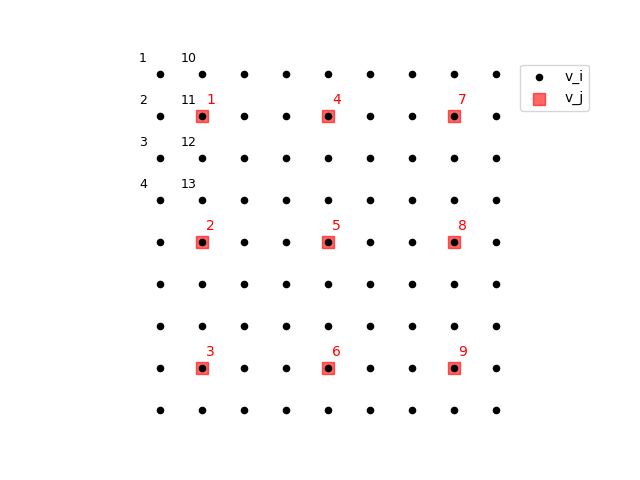
\includegraphics[scale=0.4]{figs/grid_pic.png}
    \caption{The pixel locations $v_i$ and $v_j$ for a $9 \times 9$ HR image with a downsampling factor of $3$.}
\label{fig:grid}
\end{figure}


\subsection{LR Images}
The LR images are assumed to be generated from the HR image by downsampling, applying a rotation, a shift, convolution with a point spread function (PSF). Downsampling is already implicit in the setup of the problem. To apply the other transformations, we map each $v_j$ to a shifted \& rotated center $u_j^{(k)}$ and then apply a PSF to $x$ centered on that point. 

Let $\theta_k$ denote the rotation of the $k$-th LR image around the center of the HR image. The corresponding rotation matrix is
\[
R^{(k)} =
\begin{bmatrix}
\cos(\theta_k) & -\sin(\theta_k) \\
\sin(\theta_k) & \cos(\theta_k)
\end{bmatrix}.
\]

Let $s_k \in \mathbb{R}^2$ denote the 2D shift of the $k$-th LR image relative to the HR image. Define $\bar v$ to be the center of the HR grid, which corresponds to the average of the $v_i$.

Then, each LR pixel coordinate $v_j$ maps to a corresponding location $u_j^{(k)}$ in the HR image via
\[
u_j^{(k)} = R^{(k)} (v_j - \bar{v}) + \bar{v} + s_k.
\]

See Figure \ref{fig:shift_grid} for an example of this transformation. The figure shows this transformation applied to a single pixel $j$ in a single LR image. For \textit{all} pixels in \textit{all} LR images, this transformation would need to be applied to each $j \in \{1...M\}$ and for each $k \in \{1 .. K\}$. 

\begin{figure}[h]
    \centering
    
\includegraphics[scale=0.6]{figs/grid_shift_pic.png}
    \caption{Example transformation of a pixel $j$ in one of the LR images into its shifted \& rotated center $u_j^{(k)}$.}
    \label{fig:shift_grid}
\end{figure}

Finally, the intensity of each LR pixel is modeled as a weighted average of nearby HR pixels using a point spread function (PSF). Specifically, we define
\[
y^{(k)}_j = \sum_{i=1}^{N} W_{j,i}^{(k)} \, x_i + \varepsilon_{j}^{(k)},
\]
where $\varepsilon_{j}^{(k)}$ is noise $\sim \mathcal{N}(0, \sigma^2)$, and the weights $W_{j,i}^{(k)}$ are determined by the PSF:
\[
\tilde W_{ji}^{(k)} = \exp\left(-\frac{\| v_i - u_j^{(k)} \|^2}{\gamma^2}\right).
\]
for some width parameter $\gamma$ to be learned. We then normalize:
\[
W_{ji}^{(k)} = \tilde W_{ji}^{(k)} / \sum_{i'}\tilde W_{ji'}^{(k)}
\]
We can simplify the notation by concatenating all vectors $y^{(k)} \in \mathbb{R}^M$ into a single vector $y \in \mathbb{R}^{KM}$, and likewise concatenating $W^{(k)}$ and $\epsilon^{(k)}$ into $W$ and $\epsilon$. The transformation can then be written as:
\begin{equation}
y = Wx + \epsilon, \qquad \epsilon \sim \mathcal{N}(0, \sigma^2 I)
\label{eq:forward}
\end{equation}
\subsection{MAP Reconstruction}
We seek to recover the value $x$ from the observations $y$. To do this, we take a Bayesian approach and place on $x$ a Gaussian process prior
\[
p(x) = \mathcal{N}(0, Z_x),
\]
with covariance
\[
Z_x(i,j)
=
A \exp\left\{
-\frac{\lVert v_i - v_j \rVert^2}{r^2}
\right\}.
\]
for fixed hyperparameters $A$ and $r$.
Using Equation \ref{eq:forward} and denoting $\theta = (\theta_1,\ldots,\theta_K)$ and $s = (s_1,\ldots,s_K)$, we can then derive the simple likelihood:
\begin{equation}
    p(y \mid x, s, \theta, \gamma) \propto \exp\left\{ -\frac{1}{2\sigma^2}||Wx - y||^2\right\}
    \label{eq:likelihood}
\end{equation}
We can thus form the posterior over all of the unknowns $x, \theta, \gamma$ and $s$ as:
\begin{equation}
    p(x, s, \theta, \gamma \mid y) \propto p(y \mid x, s, \theta, \gamma) \cdot p(x)
    \label{eq:post}
\end{equation}
since only $p(x)$ has an associated prior. The MAP approach maximizes this expression with respect to the unknown parameters, yielding -- after taking the log of Equation \ref{eq:post} and dropping constants -- the optimization: 
\begin{equation}
    \min_{s, \theta, x, \gamma} \frac{1}{\sigma^2} ||Wx - y||^2 + x^T Z_x^{-1}x
    \label{eq:opt1}
\end{equation}
where $W$ is a function of $s, \theta$ and $\gamma$. 

\subsection{Bayes Reconstruction}
The paper's novel work argues that this MAP methodology doesn't take into account the uncertainty in determining the high-resolution image and the consequential effects on the registration parameters. Therefore, they propose marginalizing $x$ out of the likelihood expression in Equation \ref{eq:likelihood}: 
\begin{equation*}
    p(y \mid s, \theta, \gamma) = \int p(y \mid x, s, \theta, \gamma) \ p(x) \ dx = N(0, Z_y)
\end{equation*}
with 
\[
Z_y = \sigma^2I + WZ_xW^T
\]
After some algebra, we get that maximizing this likelihood is equivalent to the following optimization:
\begin{equation}
    \min_{s, \theta,\gamma} \frac{1}{\sigma^2} ||W\mu - y||^2 + \mu^TZ_x^{-1}\mu - \log{|\Sigma|}
\end{equation}
with 
\[
\Sigma
=
\left(
Z_x^{-1}
+
\frac{1}{\sigma^2} W^T W
\right)^{-1}
\]

\[
\mu
=
\frac{1}{\sigma^2}
\Sigma W^T y
\]
Note that this $\mu$ and $\Sigma$ correspond to the mean and covariance of the Gaussian posterior distribution. 

Once the parameters $s, \theta, \gamma$ are found after optimizing the above, we fix $W$ in Equation \ref{eq:opt1} and optimize the expression solely over $x$, which gives $x^* = \mu$. 

\section{Experiments \& Results}
\subsection{Optimization Setup}
\label{sec:optimization}
We evaluate the performance of both the MAP and Bayesian reconstruction methods on synthetically generated data. The primary goal of these experiments is to assess how accurately each method can recover a high-resolution (HR) image from multiple low-resolution (LR) observations under controlled transformations.

Although the paper uses an HR image of size $384 \times 256$, we use a HR image of size $128 \times 128$ due to memory constraints. All experiments were run on an NVIDIA RTX A6000 GPU with 48 GB VRAM; using HR images larger than $128 \times 128$ resulted in the memory crashing. 


We set the other hyperparameters as specified in the paper: downsample factor $d$ = 4 (so each $LR$ image is of size $32 \times 32$), number of LR images $K = 16$, shift range $[-2, 2]$, rotation range $[-4, 4]$ in degrees, PSF width $\gamma = 2.0$, Gaussian Process width and variance $r = 1.0, A = .04$, and noise variance $\sigma^2 = .05$. 

\begin{figure}[h!]
    \centering
    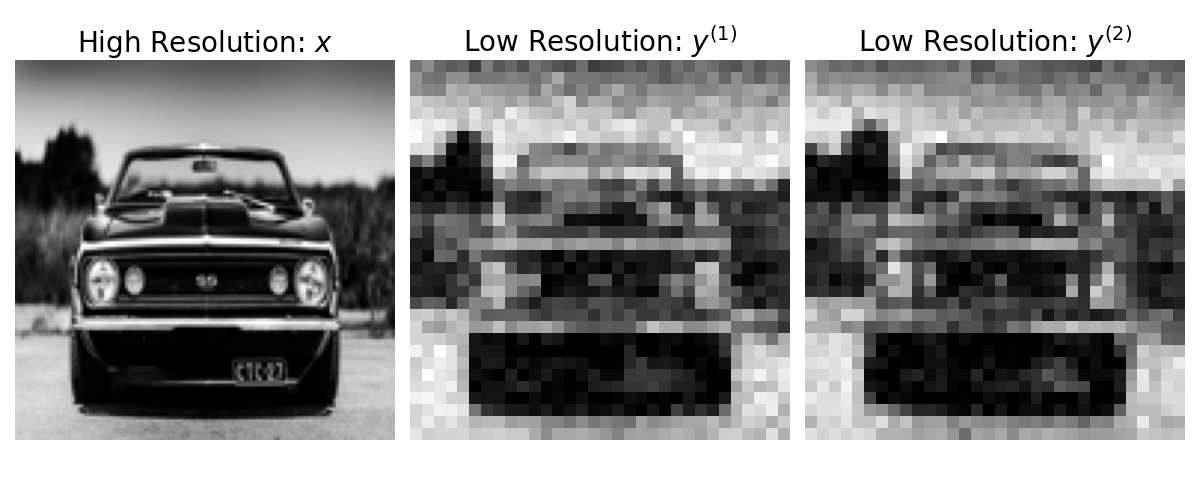
\includegraphics[width=\linewidth]{figs/hr_lr.png}
    \caption{From left to right: the HR image ($x$), and two examples low resolution images $y^{(1)}$ and $y^{(2)}$.}
    \label{fig:hr_lr}
\end{figure}
See Figure \ref{fig:hr_lr} for the HR image and synthetically generated LR images using the setup above.   

The optimization was carried out in PyTorch using the LBFGS optimizer, which approximates second-order curvature information \cite{lbfgs_wikipedia}. As done in the paper, we first optimize only the shifts, then we optimize both shifts and rotations, and finally we optimize shifts, rotations and PSF width, in each case running until a suitable convergence tolerance is reached. We include the loss plots in Appendix \ref{sec:loss_plots} for reference. 

\subsection{Patching}
In addition, as was done in the paper, we optimize the Bayesian model using only a subpatch of the LR images (to save memory / time). The paper does not specify whether the MAP model was trained using only patches of the full-sized image, so we experiment using both (\textit{MAP Full} and \textit{MAP Patch}). We use a patch size of $9$ pixels around the center of the LR image, like the original paper. 
\subsection{Results}

In this section, we detail and compare results of the Bayes and MAP methods using the setup described above. First, we show example reconstructions from both methods in Figure \ref{fig:recons}.

\begin{figure}[h]
    \centering
    
\includegraphics[width=\linewidth]{figs/recons.png}
    \caption{Reconstruction of the HR using Bayes \& MAP methods.}
    \label{fig:recons}
\end{figure}

It is not entirely obvious which reconstruction is best. The MAP Full reconstruction appears to have a smoother, more blended look to it, while the Bayes and MAP Patch reconstructions seem to have higher sharpness in certain areas but more of a grainy texture. 

We also assess these reconstructions quantitatively by comparing the found rotation/shift/gamma parameters to their ground truths. 
See Figures \ref{fig:gamma}, \ref{fig:rot_error}, and \ref{fig:shift_error} for the results. 
\begin{figure}[h]
    \centering
    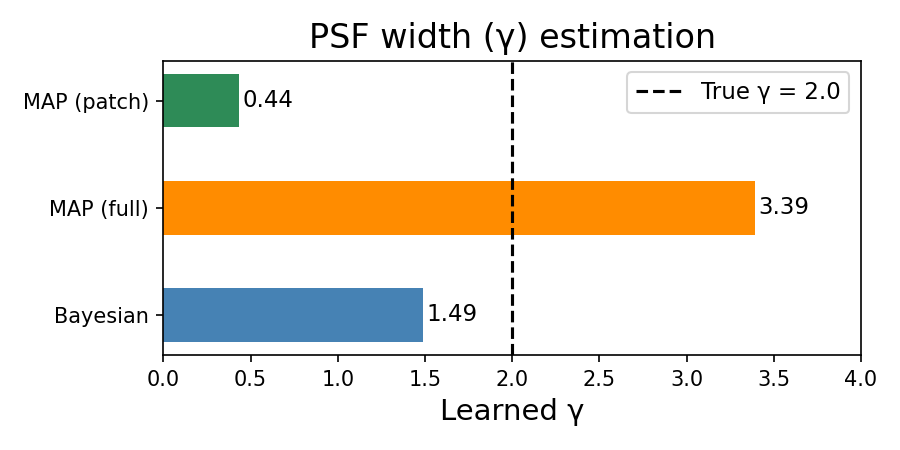
\includegraphics[width=\linewidth]{figs/gamma_comparison.png}
    \caption{Comparison between the predicted $\hat \gamma$ values and the ground truth.}
    \label{fig:gamma}
\end{figure}

\begin{figure}[h]
    \centering
    
\includegraphics[width=\linewidth]{figs/rotation_abs_error_deg.png}
    \caption{Absolute error between ground truth and estimated rotations for each low-resolution image.}
    \label{fig:rot_error}
\end{figure}

\begin{figure}[h]
    \centering
    
\includegraphics[width=\linewidth]{figs/shift_2d_comparison.png}
    \caption{Shift error between ground truth and estimated rotations for each low-resolution image. Lines are drawn connecting the estimates to their corresponding ground truths.}
    \label{fig:shift_error}
\end{figure}
The Bayesian method learns the closest $\hat{\gamma}$ to the true value, whereas the other two methods exhibit significantly larger errors. Since $\gamma$ controls the width of the PSF, this explains why the Bayesian reconstruction appears sharper: it underestimates $\gamma$. Conversely, the MAP (full) reconstruction appears smoother because it overestimates $\gamma$. In contrast, however, MAP (full) provides substantially better shift and rotation estimates than the Bayesian method. 

We summarize the results in Table \ref{tab:model_errors}. Note the total time it took to run the optimization for each method was on the order of $5-10$ minutes.

\begin{table}[h]
    \centering
    \small
    \setlength{\tabcolsep}{4pt}
    \begin{tabular}{lccc}
        \hline
        Method & $\gamma-\hat{\gamma}$ & Avg. shift err. & Avg. rot. err. ($^\circ$) \\
        \hline
        Bayesian    & \textbf{0.51} & 0.36 & 0.71 \\
        MAP (full)  & -1.39 & \textbf{0.22} & \textbf{0.27} \\
        MAP (patch) & 1.56 & 0.42 & 0.53 \\
        \hline
    \end{tabular}
    \caption{Estimated $\gamma$ error, average shift error, and average rotation error for each method. Bold represents the lowest in each column. }
    \label{tab:model_errors}
\end{table}

\subsection{Comparison to Paper's Results}
We found that our results were more ambiguous than the clear out-performance of the Bayesian method over the MAP method reported in the paper (see Appendix \ref{sec:original_paper}). We have two main hypotheses for this discrepancy.

First, our implementation of the paper's methods may differ from the authors' implementation, either because of bugs in our code or because of unintended deviations from their procedure. Although we spent substantial time testing our results and experimenting with different hyperparameter choices, implementation errors remain possible. Second, due to memory constraints, we used an HR image of size $128 \times 128$ rather than the $384 \times 256$ image used in the paper. It is possible that the Bayesian method performs much better relative to the other methods at larger image sizes.
\section{Conclusion}

In this project, we replicated the Bayesian image super-resolution framework of Tipping and Bishop and compared it against MAP-based reconstruction methods on synthetically generated low-resolution images. 

Overall, our results were mixed rather than showing a clear advantage for the Bayesian method. The Bayesian approach estimated the PSF width $\gamma$ most accurately and produced a visually sharper reconstruction, but the full MAP method achieved lower average shift and rotation errors. The patch-based MAP method was less accurate overall, suggesting that this may have been what the original paper used as a baseline.  

These findings differ slightly from the stronger Bayesian advantage reported in the original paper. The discrepancy may be due to implementation differences, numerical issues, or the smaller image size required by our memory constraints. Future work should therefore focus on validating the implementation more extensively and testing the methods at larger image sizes. 

\clearpage

\section{Appendix}
\subsection{Loss Plots}
\label{sec:loss_plots}
We include the loss plots from the three optimization procedures mentioned in Section \ref{sec:optimization} in Figures \ref{fig:bayes_loss_plot}, \ref{fig:map_full_loss_plot}, and \ref{fig:map_patch_loss_plot}. The dashed lines indicate the different stages of training (shifts; shifts and rotations; shifts, rotations, and $\gamma$). 

\begin{figure}[h]
    \centering
    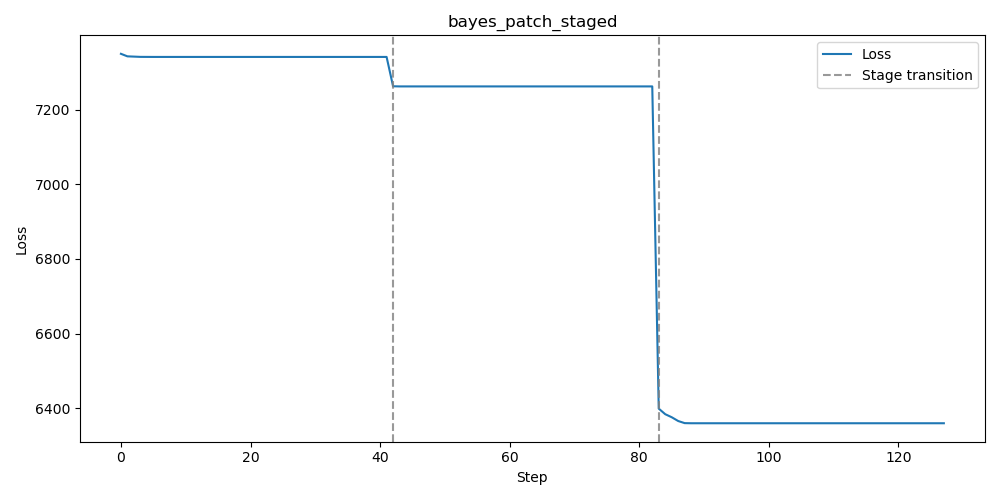
\includegraphics[width=\linewidth]{figs/bayes_loss_plot.png}
    \caption{Loss plot from optimizing the Bayesian method}
    \label{fig:bayes_loss_plot}
\end{figure}

\begin{figure}[h]
    \centering
    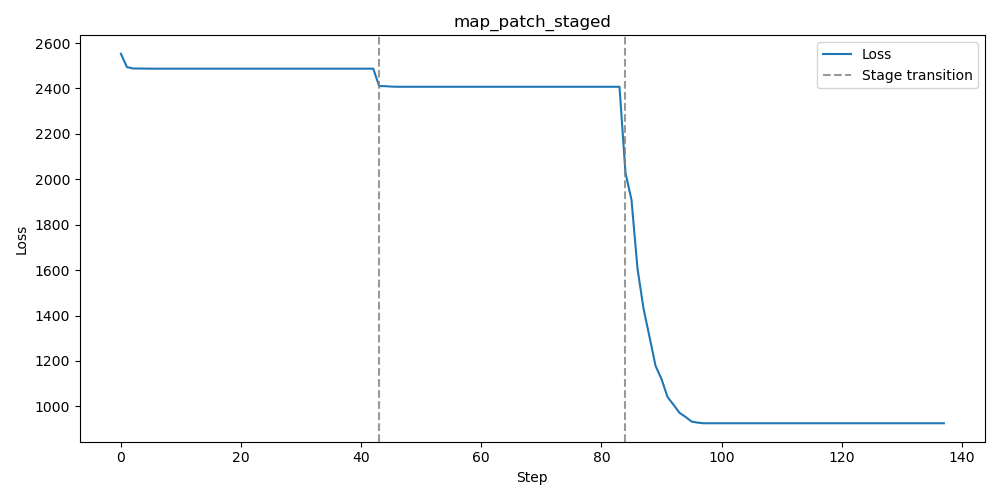
\includegraphics[width=\linewidth]{figs/map_patch_loss.png}
    \caption{Loss plot from training the MAP method on a patch of the image.}
    \label{fig:map_patch_loss_plot}
\end{figure}

\begin{figure}[h]
    \centering
    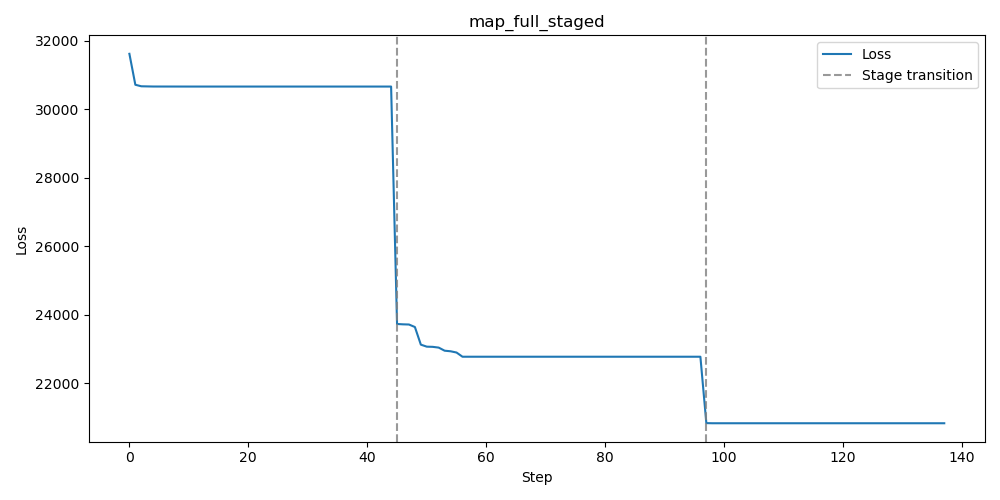
\includegraphics[width=\linewidth]{figs/map_full_loss.png}
    \caption{Loss plot from training the MAP method on the entire image.}
    \label{fig:map_full_loss_plot}
\end{figure}

\subsection{Results from Original Paper}
\label{sec:original_paper}
Figure \ref{fig:paper_results} is taken directly from the \textit{Bayesian Image Super-Resolution Paper}. It shows that the Bayesian approach predicts the registration parameters (e.g. rotation angle and shift) much better than the MAP approach. This was mostly inconsistent with our findings, although the results could be due to different hyperparameter choices or potential divergences between our implementations. However, the paper reports the converged $\hat \gamma$ value for the Bayes method was much close to the ground truth than the MAP approach ($1.94$ vs. $0.43$), which aligned with our findings well. 

\begin{figure}[h]
    \centering
    \includegraphics[width=\linewidth]{additional_figs/paper_results.png}
    \caption{Results figure taken directly from the Bayesian Image Super-Resolution paper.}
    \label{fig:paper_results}
\end{figure}

\bibliographystyle{unsrtnat}
\bibliography{references}    % This looks for references.bib
\end{document}
